\chapter{The Large Hadron Collider and the \ATLAS Detector}
\label{chap:detector}

\chapterquote{I'm not concerned about all hell breaking loose, but that a PART of hell will break loose\dots it'll be much harder to detect.}{George Carlin}

\section{Overview}
The Large Hadron Collider (\LHC) at \CERN has extended the frontiers of particle physics through its unprecedented energy and luminosity.
In 2010, the \LHC collided proton bunches, each containing more than $10^{11}$ particles, 20 million times per second, providing \unit{7}{\TeV} proton-proton collisions at instantaneous luminosities of up to \peakLumi.
A diagrammatic view of the \CERN accelerator complex is shown in \FigureRef{fig:detector:cern_accelerators}

\begin{figure}[htpb]
  \includegraphics[width=\hugefigwidth]{chapters/detector/cernaccelerators.jpg}
  \caption{Overview of the \CERN accelerator complex~\cite{CERN:2012:accelerators}: a succession of particle accelerators that are used to reach sequentially higher energies. Each accelerator boosts a beam of particles, before injecting it into the next one in the sequence. Protons, obtained through ionising hydrogen atoms, are injected from the linear accelerator (LINAC2) into the PS Booster, then the Proton Synchrotron (PS), followed by the Super Proton Synchrotron (SPS), before finally reaching the Large Hadron Collider (\LHC) ring. Protons circulate in the \LHC ring for 20 minutes before reaching their maximum energy.}
  \label{fig:detector:cern_accelerators}
\end{figure}

The high interaction rates, radiation doses, particle multiplicities and energies, when combined with the requirements for precision measurements, have set new standards for the design of particle detectors.
\ATLAS~\cite{ATLAS:2008:detector} is one of two general purpose detectors at the \LHC that have been built to probe proton-proton and heavy ion collisions.

\section{The \ATLAS Detector}
The \ATLAS detector, shown in \FigureRef{fig:detector:atlas_full_detector}, is divided into different detector subsystems, among them the tracker, the calorimeter system, the minimum bias trigger scintillators and the muon system.
This thesis deals mainly with the calorimeter and will therefore only briefly mention other detector components.

\begin{figure}[htpb]
  \includegraphics[width=\largefigwidth]{chapters/detector/AtlasDetector.CERN0803012_01.jpg}
  \caption{Overview of the full \ATLAS detector showing the four major subsystems, with human figures to scale~\cite{CERN:2012:AtlasDetector}. The inner detector, consisting of the SCT and TRT, measures the momentum of charged particles. The calorimeter systems, the LAr EM, endcap and forward calorimeters, together with the tile calorimeters, measure the energies of interacting particles. The muon chambers, on the outer edges of the detector, identify muons and measure their momenta. The solenoid and toroid magnet systems bend charged particles, allowing for greater precision in momentum measurement.}
  \label{fig:detector:atlas_full_detector}
\end{figure}

The inner (tracking) detector has complete azimuthal coverage and spans the pseudorapidity\footnote{\ATLAS uses a right-handed coordinate system with the origin taken at the nominal interaction point (IP) in the centre of the detector, the positive $x$-axis pointing inwards towards the centre of the \LHC ring and the positive $y$-axis pointing upwards. The side of the detector with positive $z$ is termed side-A while the negative $z$ side is known as side-C. Cylindrical coordinates $(r, \theta)$ are used in the transverse plane, with $\phi$ the azimuthal angle around the beam axis. The pseudorapidity and rapidity are defined as discussed in \SectionRef{sec:bg-theory:coordinates}. Distances, \DeltaR, in the pseudorapidity-azimuthal angular space are defined as $\DeltaR = \sqrt{\DeltaEta^2 + \DeltaPhi^2}$.} range $\absEta<2.51$.
In this region, where the track density is large, the desired high-precision measurements require excellent resolution of momenta and of vertex positions.
In order to make these high-granularity measurements, a variety of tracking technologies are used. Layers of silicon pixel detectors, silicon microstrip detectors (SCT) and straw tube transition radiation tracking detectors (TRT) are all are surrounded by a solenoid magnet that provides a uniform magnetic field of \unit{2}{\tesla}.
This allows tracks with $\pT \leq \unit{500}{\MeV}$ to achieve resolutions of between 0.4\% and 1\% depending on location in \pseudorap. Additionally, tracks with $\pT < \unit{500}{\MeV}$ have resolutions of between 0.1\% and 2\%, again depending on their \pseudorap~\cite{ATLAS-CONF-2010-009}.

The \ATLAS muon spectrometer, covering the pseudorapidity range $\absEta<2.7$, can identify and reconstruct muons without input from any other subdetectors.
As muons are the only interacting particles that can reliably pass through the calorimeter systems without stopping, they can be cleanly detected in the surrounding spectrometer.
A series of drift tubes are used to detect the magnetic deflection of muon tracks while and cathode strip chambers provide precision position measurements.
Overall, this system aims to identify muons with momenta between \unit{3}{\GeV} and \unit{1}{\TeV}.

The Minimum Bias Trigger Scintillators (MBTS) aim to select soft collisions between two interacting protons.
The scintillators are mounted on the inner surface of the liquid argon (LAr) end-cap cryostats and cover a pseudorapidity range of $2.12 \leq \absEta < 3.85$.
The MBTS system is constructed from \unit{2}{\centi\metre} polystyrene-based scintillator counters, 16 on each side of the detector, which, between them, cover the full azimuthal range.

\subsection{Calorimeter Overview}
\label{sec:detector:calorimeter_systems}
\begin{figure}[htpb]
  \includegraphics[width=\largefigwidth]{chapters/detector/ATLASCalorimeters.jpg}
  \caption{Cross-sectional overview of the \ATLAS calorimeter systems~\cite{ATLAS:2008:detector}. The LAr-based electromagnetic, forward and hadronic end-cap calorimeters are shown in brown, while the hadronic tile calorimeters are shown in gray and green.}
  \label{fig:detector:atlas_calorimeters}
\end{figure}

\FigureRef{fig:detector:atlas_calorimeters} shows an overview of the sampling calorimeters at \ATLAS.
The calorimeter systems cover the full range, $\absEta<4.9$, although different techniques must be used in different \pseudorap regions, due to the varying radiation environment and the requirements of the physics processes of interest. 

\begin{figure}[htpb]
  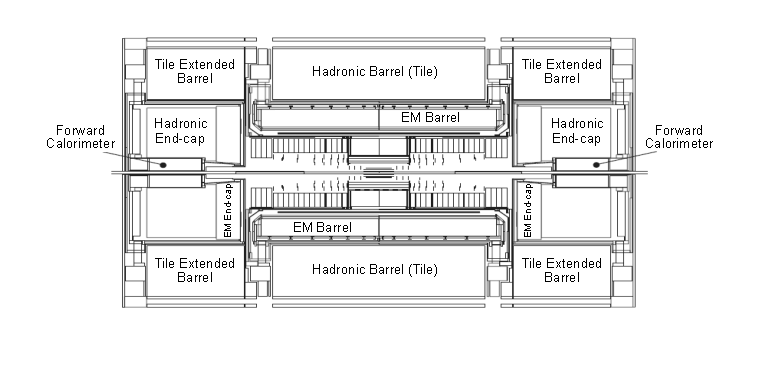
\includegraphics[width=\largefigwidth]{chapters/detector/ATLASCalorimetersFlat.eps}
  \caption{Schematic transverse view ($r$-$z$ view) of the calorimeters in the \ATLAS detector~\cite{ATLAS:2008:detector}. A cylindrical coordinate system is used, with the $z$-axis along the proton-beam.}
  \label{fig:detector:atlas_calorimeters_flat}
\end{figure}

High granularity liquid-argon (LAr) electromagnetic (EM) sampling calorimeters cover the range $\absEta < 3.2$.
In the range $\absEta < 1.7$, the hadronic calorimetry is provided by a scintillator-tile calorimeter.
This is separated into a large central barrel and two smaller extended barrel cylinders, one on either side of the main barrel.
In the end-caps, $\absEta > 1.5$, LAr technology is again used for the hadronic calorimeters, matching the outer \absEta limits of the end-cap electromagnetic calorimeters.
The LAr forward calorimeters extend out to $\absEta = 4.9$, providing both electromagnetic and hadronic energy measurements.

For the inner detector, $\absEta<2.5$, the EM calorimeter is fine-grained to allow precision measurements of electrons and photons to be made.
The other calorimeters in this region are coarser grained, although still possess sufficient resolution to satisfy the physics requirements for jet reconstruction and measurement of \ETmiss.

Calorimeter depth is an important design consideration: the calorimeters must contain electromagnetic and hadronic showers and limit punch-through into the muon system.
Electromagnetic showers are characterised by their narrow lateral profiles and are longitudinally parameterised by their radiation length $X_0$.
Hadronic showers usually have a larger transverse spread and their nuclear interaction length, $\lambda$, is typically an order of magnitude greater than $X_0$, although this is material-dependent.

The barrel of the EM calorimeter is more than \unit{22}{X_0} thick, while the thickness of the end-cap is more than \unit{24}{X_0}.
For high energy jets, the active calorimeter comprises \unit{9.7}{\lambda} in the barrel and \unit{10}{\lambda} in the end-caps; providing adequate resolution.
\FigureRef{fig:detector:deadMaterial} shows the total amount of material, including non-instrumented sections, in units of $\lambda$, as a function of \absEta.
Taking all of this into account, the total thickness, as demonstrated using test beams, is sufficient to reduce punch-through below the level of prompt or decay muons.
Together with the large \pseudorap coverage, this also ensures a good \ETmiss measurement, which is a particularly important signature for those analyses looking for evidence of supersymmetry. 

\begin{figure}[htpb]
  \includegraphics[width=\largefigwidth]{chapters/detector/deadMaterial.eps}
  \caption{Cumulative amount of material in the \ATLAS detector, in units of interaction length, $\lambda$, as a function of \absEta. The coverage from each individual calorimeter component is shown separately, while the sections closest to the interaction point, which are not instrumented for calorimetry, are shown in brown~\cite{ATLAS:2008:detector}.}
  \label{fig:detector:deadMaterial}
\end{figure}

\subsection{Liquid Argon Electromagnetic Calorimeter}
The electromagnetic calorimeter barrel, $\absEta < 1.475$, and end-caps, $1.375 < \absEta < 3.2$, are each housed in their own cryostat.
The central solenoid, located in front of the electromagnetic calorimeter, is a significant source of dead material - approximately \unit{1}{\lambda} at its greatest extent, restricting the maximal achievable calorimeter performance.
Placing the solenoid and the liquid argon calorimeter inside a single vacuum vessel mitigates this effect by eliminating two vacuum walls which would otherwise be required.
The barrel calorimeter consists of two identical half-barrels, separated by a \unit{4}{\milli\metre} gap at $\pseudorap = 0$.
The two end-cap calorimeters are each subdivided into two coaxial wheels: the outer wheel covering the region $1.375 \leq \absEta < 2.5$ and the inner wheel $2.5 \leq \absEta < 3.2$.

The electromagnetic calorimeter is a lead-LAr detector with lead absorber plates along its full coverage and readout provided by accordion shaped electrodes.
This accordion geometry avoids the necessity for azimuthal cracks, providing complete symmetry in $\phi$.
For $\absEta < 2.5$, the region instrumented for precision physics, the calorimeter is segmented in depth into three longitudinal layers, numbered from 1 to 3 outwards from the beam axis.
Outside this region, the end-cap inner wheel is divided into only two sections in depth and also has a coarser lateral granularity.

A presampling detector is installed for $\absEta < 1.8$ in order to allow the energy lost by electrons and photons upstream of the calorimeter to be measured and corrected for.
This consists of an active LAr layer which is \unit{1.1}{\centi\metre} thick in the barrel region, and \unit{0.5}{\centi\metre} thick in the end-cap.

\subsection{Hadronic Calorimeters}
\subsubsection{Tile Calorimeter}
As can be seen in \FigureRef{fig:detector:atlas_calorimeters_flat}, the tile
calorimeter is located outside the electromagnetic calorimeter, extending radially from
\unit{2.28}{\metre} to \unit{4.25}{\metre}. It is a sampling calorimeter,
consisting of steel absorbing plates interleaved with scintillating tiles, which provide the
active material. The hadronic barrel covers $\absEta < 1.0$ and is complemented
by two extended barrels covering $0.8 \leq \absEta < 1.7$; each of these
subdetectors is divided azimuthally into 64 modules in $\phi$.

Similarly to the electromagnetic calorimeter, the tile is segmented into three layers:
approximately 1.5, 4.1 and \unit{1.8}{\lambda} thick for the barrel and 1.5,
2.6 and \unit{3.3}{\lambda} thick in the extended barrel. Two sides of the
scintillating tiles are read out by wavelength shifting fibres into two separate
photomultiplier tubes. The readout cells, built by grouping fibres together in the
photomultipliers, are pseudo-projective towards the interaction region.

\subsubsection{Liquid Argon Hadronic End-cap Calorimeter}
The Hadronic End-cap Calorimeter (HEC) is a copper detector consisting of two
independent wheels per end-cap, located directly behind the end-cap
electromagnetic calorimeter (\FigureRef{fig:detector:atlas_calorimeters_flat})
and sharing the same LAr cryostats. The HEC covers the region $1.5 \leq \absEta < 3.2$,
overlapping with both the tile calorimeter and the forward calorimeter.

Each of the HEC wheels, which span $0.475 \leq r < \unit{2.03}{\metre}$,
is divided into 32 identical wedges in $\phi$ and two segments in depth, giving
four layers per end-cap in total. The wheels closest to the interaction point
are built from \unit{25}{\milli\metre} parallel copper plates, while those
further away use \unit{50}{\milli\metre} copper plates: in each case the first
of these plates is half-thickness. As the HEC is a sampling calorimeter, the copper plates
are interleaved with \unit{8.5}{\milli\metre} gaps filled with liquid argon,
which provides the active medium.

\subsection{Liquid Argon Forward Calorimeter}
The Forward Calorimeter (FCAL) consists of one module at either end of the
detector, approximately \unit{10}{\lambda} deep, providing coverage for the
region $3.2 \leq \absEta < 4.9$. It is integrated into the end-cap cryostats
although recessed by about \unit{1.2}{\metre} from the electromagnetic calorimeter;
because of the limited available depth a high-density design is required. The two
FCALs each contain three modules: a copper calorimeter, optimised for electromagnetic
measurements, and two tungsten calorimeters, predominantly aiming to perform
hadronic measurements. Each module has the form of a matrix, with regularly
spaced longitudinal channels filled with concentric tubes, parallel to the beam
axis. Each tube contains a rod, and is otherwise filled with liquid argon which
acts as the sensitive medium.

\section{Detector Performance}
\subsection{Single Hadron Detector Response}
\label{sec:detector:single-particle}
The response of the calorimeters to isolated charged hadrons can be examined by
considering the ratio of the energy, $E$, deposited in the calorimeter to the momentum,
$p$, of the associated track. Comparing the \angles{E/p} distribution in data and
\MC allows an evaluation to be made of the modelling uncertainty on the calorimeter
response in \MC. \FigureRef{fig:detector:single-particle-response} shows
\angles{E/p} as a function of track momentum for two different bins in \absEta,
after background subtraction. The agreement between data and \MC simulation is
within $\sim2\%$ for particles with momenta in the \unit{1-10}{\GeV} range, increasing
to around 5\% for momenta in the \unit{10-30}{\GeV} range.

\begin{figure}[htpb]
  \subfloat[$\absEta < 0.6$]{
    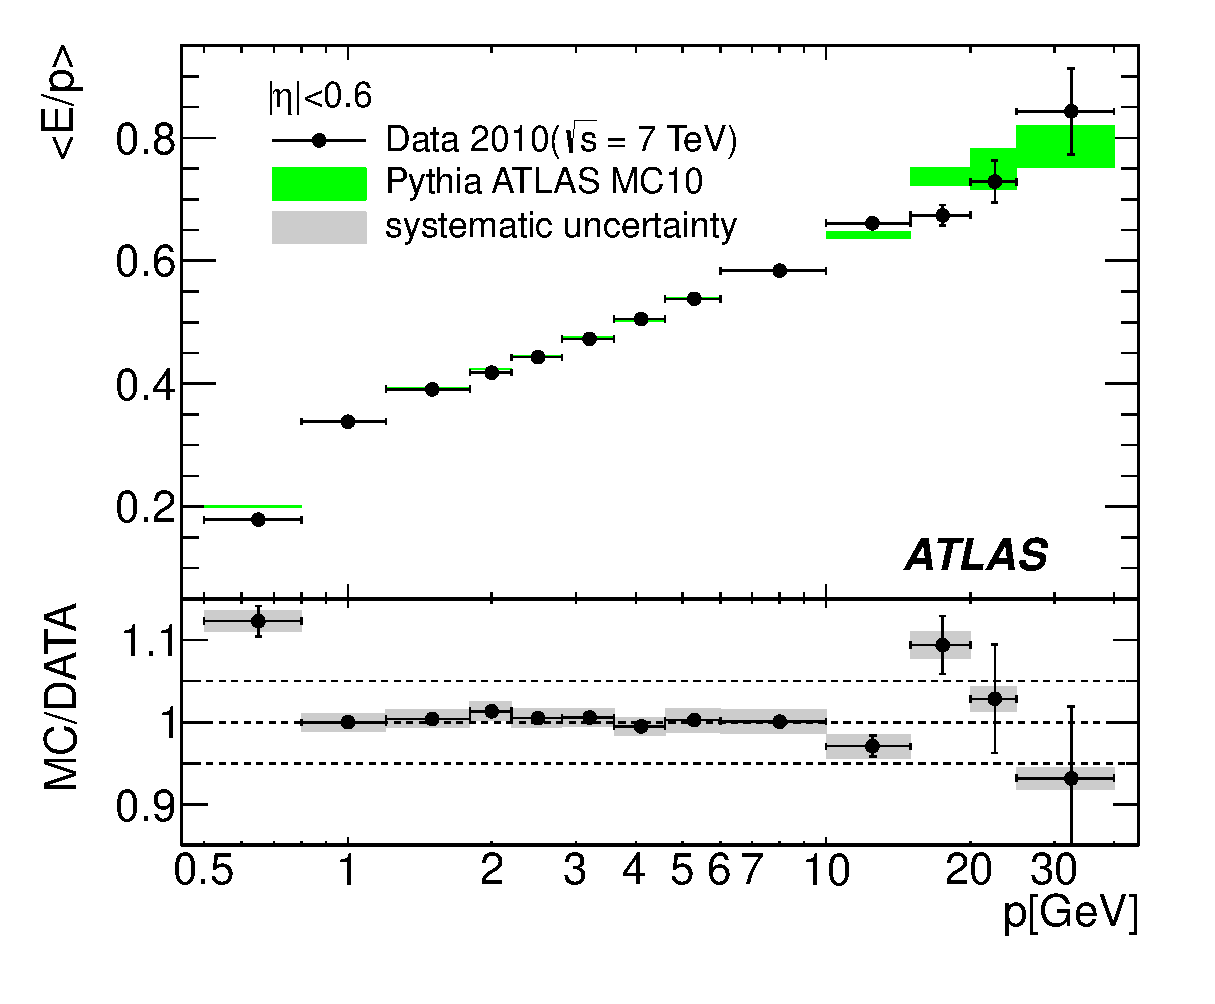
\includegraphics[width=\smallfigwidth]{chapters/detector/SingleParticleEoverP.7TeV.eta0.6.eps}
    \label{fig:detector:single-particle-response_central}}
  \quad
  \subfloat[$0.6 \leq \absEta < 1.1$]{
    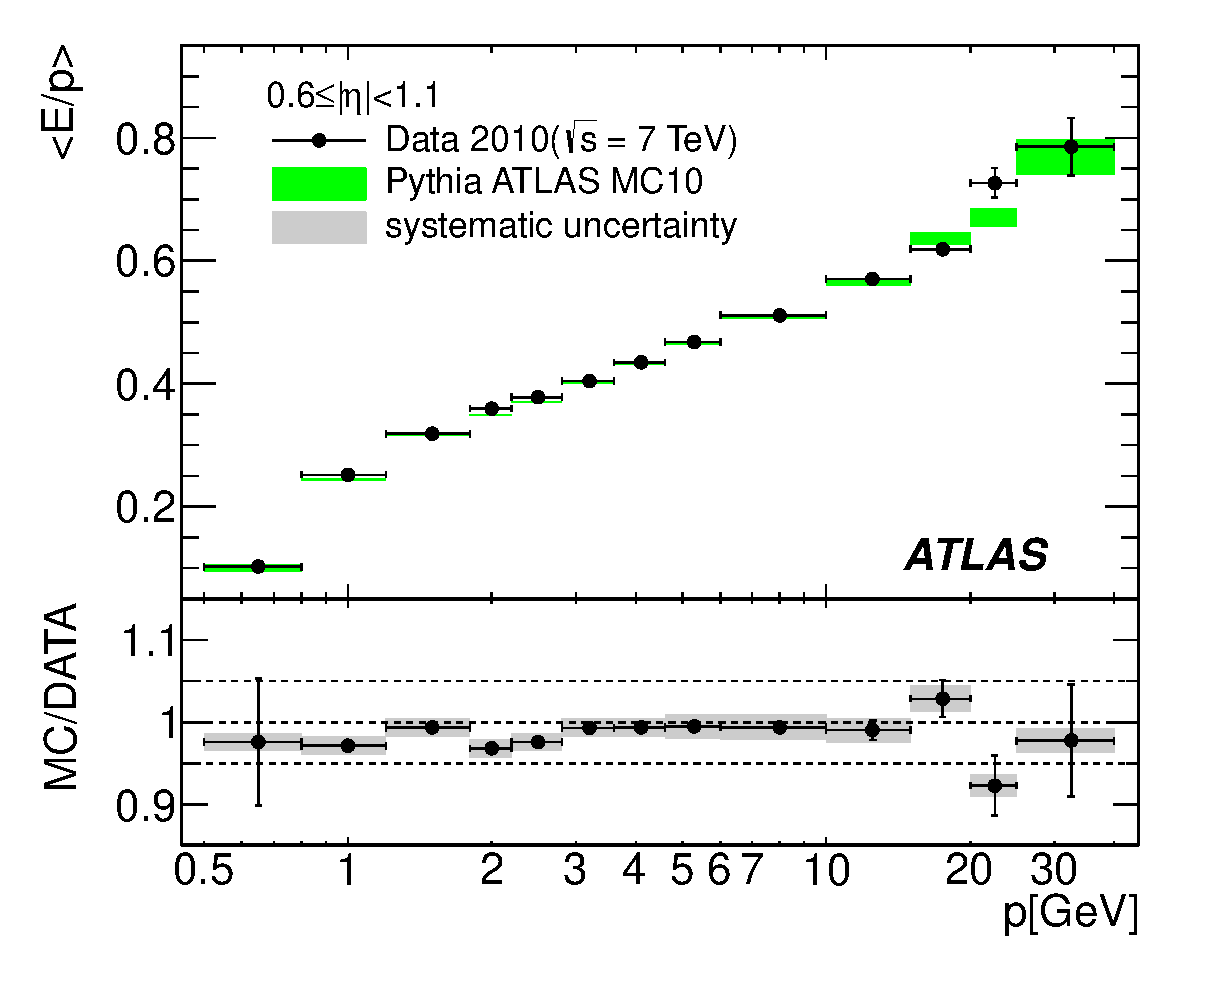
\includegraphics[width=\smallfigwidth]{chapters/detector/SingleParticleEoverP.7TeV.0.6eta1.1.eps}
    \label{fig:detector:single-particle-response_forward}}
  \caption{\angles{E/p} as a function of the track momentum for \protect\subref{fig:detector:single-particle-response_central} central and \protect\subref{fig:detector:single-particle-response_forward} more forward tracks. The black markers represent $\rootS = \unit{7}{\TeV}$ collision data, while the green rectangles show the \MC prediction, with the vertical width indicating the associated statistical uncertainty. The lower sections show the ratio of the \MC simulation prediction to collision data. The grey band indicates the size of the systematic uncertainty on the measurement~\cite{CERN-PH-EP-2012-005}.}
  \label{fig:detector:single-particle-response}
\end{figure}

\subsection{Jet Energy Resolution}
\label{sec:detector:jer}
Fully calibrated jets, see \SectionRef{sec:analysis-tools:jet_reconstruction} for
details, reconstructed using the \akt algorithm with $R=0.6$ are used to study
the jet resolution. Two different methods are used here: the first coming from \dijet
\pT balancing and the second from constructing quantities parallel and transverse
to the \dijet system, known as the bisector technique. For jets with $\absRap < 2.8$,
the results from these two methods are found to be consistent in both data and \MC. 

\begin{figure}[htpb]
  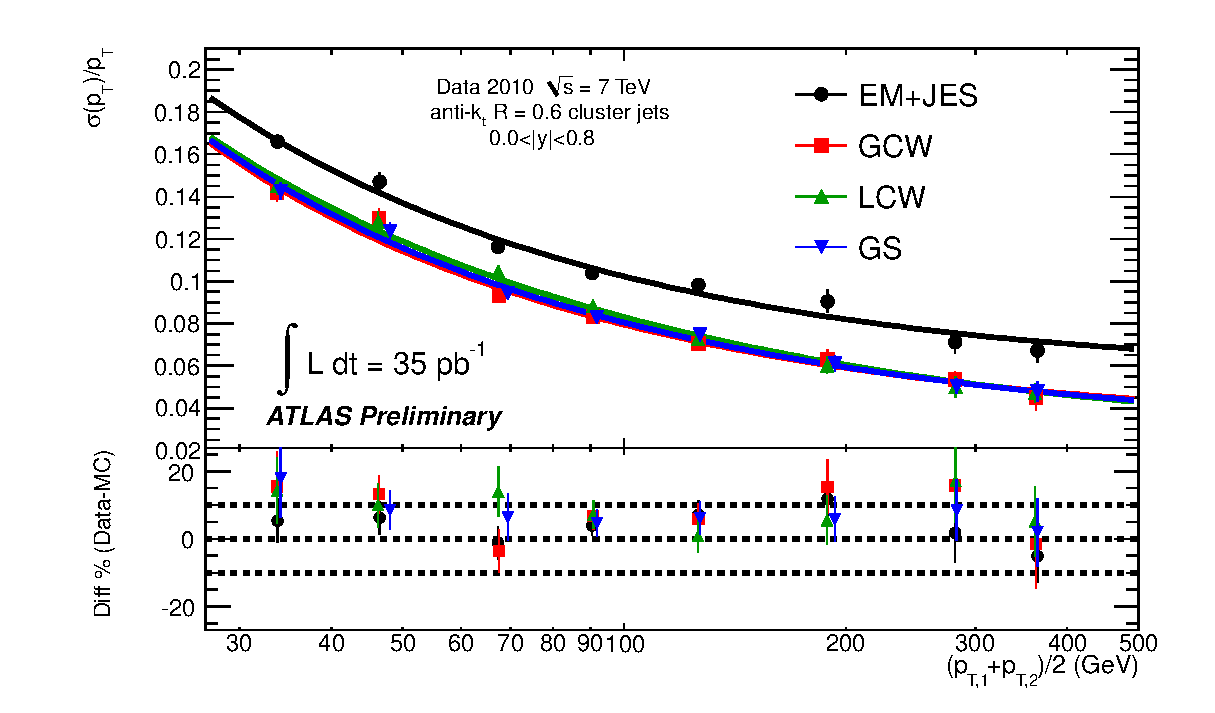
\includegraphics[width=\largefigwidth]{chapters/detector/JERDiffJESDataMC.0.6.eps}
  \caption{Fractional jet energy resolution as a function of average \dijet \pT
           for four different jet calibration schemes: the EM+JES, Global Cell Weighting
           (GCW), Local Cluster Weighting (LCW) and Global Sequential (GS) calibrations;
           only EM+JES has been fully validated for use in \ATLAS, although other
           calibration schemes may be used in future data taking. Lines of best
           fit are shown in each case. The lower section shows the relative difference
           between \MC and the results from data. The black dotted lines indicate
           a relative uncertainty of $\pm10\%$~\cite{ATLAS-CONF-2010-054}.}
  \label{fig:detector:jer}
\end{figure}

\FigureRef{fig:detector:jer} shows the fractional jet energy resolution as
a function of the average \pT of the \dijet system.  The calorimeter jet reconstruction
and selection efficiency relative to track jets is determined in data and \MC using
a tag and probe technique and found to be in good agreement, within systematic uncertainties,
for track jets with \pT values between 5 and \unit{40}{\GeV}~\cite{ATLAS-CONF-2010-054}.

\section{Trigger System}
\label{sec:detector:trigger}
When the design bunch spacing is reached, with collisions occurring every
\unit{25}{\nano\second}, the event rate of \unit{40}{\mega\Hz} is five orders of
magnitude greater than the rate at which data can be recorded, which is limited to 
\unit{400}{\Hz}. This means that the trigger systems must achieve an overall
rejection factor of $10^5$ while avoiding biases and retaining the highest
possible proportion of interesting events. During 2010, the bunch spacing was
kept at \unit{50}{\nano\second}, slightly easing this pressure.

The \ATLAS trigger system has three distinct levels: Level-1 (L1), Level-2 (L2),
and the event filter (EF). Each level of the trigger refines the decision made
by previous levels by applying additional, stricter selection criteria.
Initially, event information is accepted from the readout electronics and
buffered; the hardware-based L1 trigger system then uses a subset of the
available detector information to reject events: budgeting \unit{2.5}{\milli\second}
of processing time per event, it is able to reduce the overall rate to
\unit{75}{\kHz}. Events which pass the L1 trigger are then transferred to the L2
and EF trigger systems, collectively known as the high-level trigger (HLT). Each
HLT trigger is seeded from a specific lower level trigger and is able to examine
relevant features of the event in greater detail in order to make an overall
trigger decision. Events passing one or more triggers after the final,
``Physics'' decision are passed to the data acquisition system.

The central trigger processor implements a `trigger menu', comprising a list of
trigger selections together with their associated prescales; only triggers specified by
the processor are allowed to run in each event. The majority of trigger
menu items are prescaled: only recording a set proportion of otherwise acceptable
events. This allows optimal use of available bandwidth in the face of changing
luminosity conditions.

\subsection{Level-1 Trigger}
Due to the limited time available, the L1 trigger only uses a small amount of
the available detector information: namely the calorimeter and muon systems. The
aim of the L1 system is to identify high \pT leptons, photons and jets as well as events
with large \ETmiss or \ETtotal. High \pT muons are identified using trigger
chambers in the barrel and end-cap regions of the muon spectrometer, while the
identification of other interesting event features is based on reduced-granularity information from all parts of the
calorimeter system. Events which pass the L1 trigger selection are transferred to
the L2 processing system and, if accepted by the HLT, onwards to the
data acquisition systems via point-to-point links.

In each event, the L1 trigger also defines one or more Regions-of-Interest (RoIs):
the geographical coordinates in \etaphi space of those regions within the
detector where its selection process has identified interesting features. The
RoI data includes information on the type of feature identified and the criteria
passed, usually some sort of threshold. This information is passed to the HLT
for later use.

\subsection{High-Level Trigger}
The RoI information from L1 is used to seed the L2 trigger. L2 triggers are able
to use all of the available detector data in the region covered by the RoIs at
full granularity and precision; this corresponds to approximately 2\% of the
total event data. An average event processing time of \unit{40}{\milli\second}
is allowed at this stage, resulting in an output event rate of approximately
\unit{3.5}{\kHz}. The event filter performs the final stage of event selection,
implementing analysis procedures similar to those performed offline to reduce
the final event rate to roughly \unit{400}{\Hz}. In particular, EF jet triggers
implement the \akt algorithm, although this was not used to reject events during
2010.

\subsection{Jet Triggers}
Although the spectrum of jets produced is steeply falling, it would be
preferable from the point of view of physics analyses, particularly differential
cross-section measurements, to have a roughly uniform rate across the full jet
\ET spectrum. Collecting sufficient statistics across the spectrum is also
important for the measurement of detector and trigger efficiencies. Accordingly,
a series of inclusive jet triggers are used, each with a higher threshold than
the previous one. By changing the prescales of these triggers, the jet trigger
menu can be optimised to achieve a roughly flat event rate across the \ET
spectrum despite rising luminosity. The jet-trigger thresholds can also be
changed, but this is a less frequent operation.

The jet trigger is split into logically independent systems: one covering the
central region, $0 \leq \absEta < 3.2$ and one covering the forward region,
$3.2 \leq \absEta <4.9$. At Level-1, these systems use information from
different calorimeter subsystems: central trigger jets rely on information from
the electromagnetic barrel, tile and end-cap calorimeters, while forward trigger
jets use information from the forward calorimeters only. At Level-2, however, information
from multiple trigger systems may be considered, depending on the position of the
L1 RoI, while in the Event Filter, information from the whole detector is
combined~\cite{ATLAS-CONF-2010-028}.

Additionally, the Minimum Bias Trigger Scintillators (MBTS), located in front of
the end-cap cryostats and covering $2.09 \leq \absEta < 3.84$, are often used in jet-based
analyses to provide fully efficient triggering for low \pT jets. The trigger
L1\_MBTS\_1, requiring at least one hit in the minimum bias scintillators, is
the primary trigger used to select minimum-bias events in \ATLAS.

\subsection{Measurements of Trigger Efficiency from Data}
Understanding the efficiencies of relevant triggers is an important part of any
physics analysis. As little weight as possible needs to be given to techniques
relying solely on performance in \MC models; in-situ methods are much preferred.

The two major in-situ methods are the ``orthogonality'' and ``bootstrap''
methods. In each case, these rely on constructing a sample of events which can
then be examined to see what proportion of them pass the trigger of interest.
Orthogonality relies on taking events that pass a trigger which is known to be
uncorrelated to the trigger under consideration. This can, however, introduce physics
biases: muon triggers, for instance, could increase the proportion of
heavy flavour jets. Jet trigger efficiencies are therefore usually determined
using the bootstrap method in which events passing a lower threshold jet trigger,
which is known to be on plateau in the \pT region of interest, are used. Firstly,
events which pass minimum-bias triggers are used to measure the efficiency of
those triggers with the lowest \pT thresholds, then the low threshold jet
triggers are used as the baseline to select events with which to examine higher
\pT-threshold triggers.

Efficiencies can be determined either on a \emph{per-jet} or, more commonly, on
a \emph{per-event} basis. Per-event efficiencies are the fraction of events in
which at least one jet passes the appropriate trigger among all events with at
least one jet at the given \pT. Per-jet efficiencies are the fraction of jets
passing the appropriate trigger among all jets at the given \pT. Per-jet
efficiencies are more complex, due to their reliance on matching between offline
jets and trigger objects and are rarely used.

\FigureRef{fig:detector:forward_bin_trigger_efficiencies} shows per-event
trigger efficiencies for six different triggers in the region $3.6 \leq \absRap < 4.4$.
Here the characteristic serpentine shape of a typical efficiency curve can be seen, rising from zero efficiency to reach a plateau.
In \FigureRef{fig:detector:forward_bin_triggers_L1_akt4}~and~\ref{fig:detector:forward_bin_triggers_L1_akt6}
the efficiencies for L1 triggers are shown. The likelihood that a given L1
trigger will fire, before prescale, is shown as a function of offline jet \pT,
using \akt jets, with $R=0.4$ on the left and $R=0.6$ on the right. Three
different L1 thresholds are shown, each requiring a greater level of L1 \ETEM in
order to trigger. The efficiency for the lowest threshold, L1 $\ETEM > \unit{10}{\GeV}$,
must be determined using MBTS triggers, but higher thresholds can be
bootstrapped from previous jet triggers.

In \FigureRef{fig:detector:forward_bin_triggers_L1L2_akt4}~and~\ref{fig:detector:forward_bin_triggers_L1L2_akt6},
the efficiency curves for L2 triggers are shown, again as a function of offline
jet \pT. The correlation between the \ETEM threshold and the offline \pT at
which plateau is first reached is evident, as is the distinctive shape with
which efficiency rises as a function of offline \pT. Specific details relevant
to the efficiency curves shown here are discussed further in \SectionRef{sec:forward-inclusive:trigger_efficiencies}.

\begin{figure}[htpb]
  \subfloat[L1 efficiency, \akt $R=0.4$ jets]{
    \includegraphics[width=\smallfigwidth]{chapters/forward-inclusive/forward_bin_triggers_L1_akt4.eps}
    \label{fig:detector:forward_bin_triggers_L1_akt4}}
  \quad
  \subfloat[L1 efficiency, \akt $R=0.6$ jets]{
    \includegraphics[width=\smallfigwidth]{chapters/forward-inclusive/forward_bin_triggers_L1_akt6.eps}
    \label{fig:detector:forward_bin_triggers_L1_akt6}}
  \\
  \subfloat[L1+L2 efficiency, \akt $R=0.4$ jets]{
    \includegraphics[width=\smallfigwidth]{chapters/forward-inclusive/forward_bin_triggers_L1L2_akt4.eps}
    \label{fig:detector:forward_bin_triggers_L1L2_akt4}}
  \quad
  \subfloat[L1+L2 efficiency, \akt $R=0.6$ jets]{
    \includegraphics[width=\smallfigwidth]{chapters/forward-inclusive/forward_bin_triggers_L1L2_akt6.eps}
    \label{fig:detector:forward_bin_triggers_L1L2_akt6}}
  \caption{Jet trigger efficiency at L1 (top) and combined L1+L2 (bottom) as a function of
           reconstructed jet \pT for \akt jets with $R=0.4$ (left) and $R=0.6$ (right) in the
           forward region $3.6 \leq \absRap < 4.4$, shown for three different trigger thresholds in each case.
           The trigger thresholds are at the electromagnetic scale, while the jet \pT is at the
           calibrated scale (see \SectionRef{sec:analysis-tools:jet_reconstruction}). Due
           to the presence of a dead FCAL trigger tower, which spans 0.9\% of the
           \etaphi acceptance, the efficiency is not expected to reach 100\%.}
  \label{fig:detector:forward_bin_trigger_efficiencies}
\end{figure}
